\documentclass[../main]{subfiles}
\begin{document}
    \setcounter{secnumdepth}{2}
    \chapter{序論}
        \section{背景}
        近年,商業施設での清掃作業や屋外での宅配など,屋内外を問わず多くの場所で自律移動ロボットが活用されている.
        それらのロボットを安全かつ正確に運用するためには,自己位置推定をはじめとする様々な機能を持たせる必要がある.
        現在,商業施設などで活用されている自律移動ロボットは,メトリックマップと呼ばれる,あらかじめセンサで取得した
        環境の詳細なデータを持つ地図が使用されている.また,それらの地図を用いて,
        
        
        一方,人はそのような詳細な地図がなくても,「2つ目の信号で右」のような言葉の情報に基づき目的地まで移動することができる.
        そこで,そのような人の移動する能力をロボットの自律移動に応用する手法が研究されている.
        例えば,島田らは人の道案内に注目し,人の道案内の要素を取り入れたロボットのナビゲーション手法を提案した\cite{shimada_paper1}\cite{shimada_paper2}.
        この手法では,人が道案内で用いる情報をアンケートにより収集し,目的地まで移動させるナビゲーション手法を提案したc.
        
        アンケートを実施して人の道案内には「通路の特徴」を重視しているという結果を得る.
        

        人が目的地まで移
        どのような情報を必要としているのかを道案内に関するアンケートにより解析し,その情報をナビゲーションに組み込むことにより,ロボットを人の道案内のように
        目的地まで移動させるナビゲーション手法を提案した\cite{shimada_paper1}\cite{shimada_paper2}.
        
        トポロジカルマップとシナリオによるナビゲーション手法を提案した.この研究では,人が目的地まで移動する際に必要としている情報をアンケートにより取得し,
        得られた情報からナビゲーションに用いるトポロジカルマップと呼ばれる地図と,シナリオと呼ばれる人の道案内を言葉にしたものの形式を決定し,
        人の道案内のようにロボットを目的地まで移動させるナビゲーションの手法を提案した.また,提案したナビゲーション手法の有効性を実機を用いた実験により検証した.
        実験の結果,通路の認識が正しく行われた場合は,提案したナビゲーション手法により目的地に到達できるが,
        誤認識が起きた場合はロボットが経路から外れ,ナビゲーションに失敗してしまうということが報告されている.
        先行研究では,通路の認識にはLiDARを使用しており,通路の誤認識は,開いているドアや隙間にLiDARが反応したことが原因であると述べられている.
        ここで,通路の認識にカメラ画像を用いることで,誤認識を解消し,ナビゲーション途中に経路から外れるという問題を解決できるのではないかと考えた.

        \newpage

        \section{目的}
        本研究は,全天球カメラ画像に基づく通路認識の手法を提案する.そして,先行研究により提案された,実ロボットを用いた
        トポロジカルマップとシナリオに基づくナビゲーションに対し,認識した通路の特徴情報を適用することで本手法の有効性を検証する.
        検証の際は,本研究と先行研究のナビゲーション結果に着目し,その成功回数を比較することとする.


        また,本研究では\fref{figure::image_exp}に示すような,全天球カメラの標準的なフォーマットである正距円筒図法という形式で画像を扱う.

        \begin{figure}[H]
            \centering
            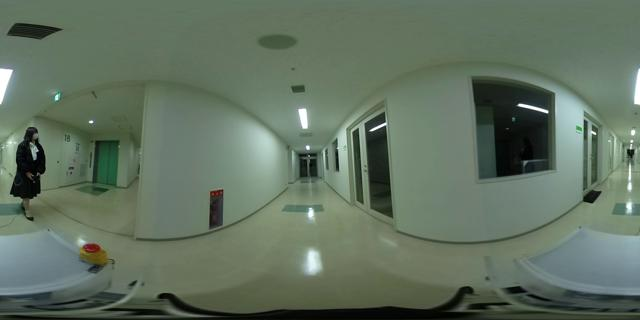
\includegraphics[width=10cm]{../images/18F_aisle_exp.jpg}
            \caption{Example of spherical camera image of equirectangular projection.}
            \label{figure::image_exp}
        \end{figure}
        
        \newpage

        \section{関連研究}
        Mueller らは GIS(Geo Information System)をベースとしたトポロジカルマップに分岐
        点の情報を組み込み,検出した分岐点の情報を自己位置推定に用いた[7].この手法では,
        分岐点にトポロジカルマップのノードが設定されている.自己位置推定の際には,分岐点
        から分岐点までの距離や,十字路などの分岐点の種類や分岐点から枝分かれする道と道の
        間の角度を用いる.なお,LiDAR を用いて生成した占有格子地図から分岐点を検出する.
        このとき,枝分かれする道の方向も同時に求める.そのため,自己位置推定に用いる情報
        として分岐点の種類に加え,分岐点から枝分かれする道の角度を用いることができる.ま
        た,自己位置推定にはパーティクルフィルタを用いている.図 1-2 にはその様子を示す.図
        1-2(a)は分岐点と枝分かれする道の方向を検出している様子である.また,図 1-2(b)はパー
        ティクルフィルタを用いた自己位置推定の様子である.


        また,澤橋らは道の分岐点をノード,道をエッジとしたトポロジカルマップを作成し,
        これを経路計画や自己位置推定に用いた自律ナビゲーションシステムを提案した[8].この
        手法では,自己位置推定を大まかな移動距離と方位からからロボットの通過したエッジの
        推定を行う.そのために,一定数保存したオドメトリの情報から直線的走行を抽出する.
        抽出した直線の長さと進んだ方位から自己位置推定を行う.ノードごとに確率を持ち,そ
        れまで進んできた軌跡から到達可能なノードの確率が高くなる方式である.この時,走行
        可能領域など,環境認識のために LiDAR やカメラから取得した意味情報を利用している.
        また,大域的経路計画の際は,初期位置と目的地を選択し,各ノードを結ぶエッジの長さ
        をコストとして,それらの和が最も小さくなるような経路を選択するよう大域経路として
        採用している.

        \section{本論文の構成}
        本論文ではまず,第1章で研究背景,目的,関連研究について述べた.第2章では,本研究で用いる要素技術について述べる.また,第3章では提案した手法について述べ,
        第4章では提案した手法の有効性の検証を行う.また,第5章では4章で行なった実験の結果をまとめ,考察を行う.最後に,第6章で本研究のまとめを行う.
\end{document}